% Meta-Diffusion: experimental record
%
% Compile:  pdflatex meta_diffusion_record.tex   (twice, for the table of contents)
% Requires: amsmath amssymb booktabs tikz xcolor hyperref caption enumitem geometry
%
% The split tree in section 2 was generated from artifacts/cifar100_domainshift.json
% by scripts/gen_tree_tex.py, so the figure cannot drift from what the code loads.

\documentclass[11pt]{article}

\usepackage[a4paper,margin=1in]{geometry}
\usepackage{amsmath,amssymb}
\usepackage{booktabs}
\usepackage{array}
\usepackage{enumitem}
\usepackage{graphicx}
\usepackage{xcolor}
\usepackage{tikz}
\usetikzlibrary{arrows.meta,positioning,calc,fit,backgrounds}
\usepackage[font=small,labelfont=bf]{caption}
\usepackage{hyperref}

\definecolor{shared}{HTML}{1D4E4A}   % shared parameters, frozen at deployment
\definecolor{coord}{HTML}{B06A14}    % the task coordinate, optimised at deployment
\definecolor{overturn}{HTML}{8C3A32} % a conclusion later overturned

\hypersetup{colorlinks=true, linkcolor=shared, urlcolor=shared, citecolor=shared}

% ---- notation shorthands -------------------------------------------------
\newcommand{\epshat}{\hat{\varepsilon}}
\newcommand{\zS}{z_{S}}
\newcommand{\zencT}{z^{\mathrm{enc}}_{T}}
\newcommand{\ztilT}{\tilde{z}_{T}}
\newcommand{\zstarT}{z^{\star}_{T}}
\newcommand{\Dss}{D^{s}_{y,S}}
\newcommand{\Dqs}{D^{q}_{y,S}}
\newcommand{\Dst}{D^{s}_{y,T}}
\newcommand{\Dqt}{D^{q}_{y,T}}
\newcommand{\KT}{K_{T}}
\newcommand{\MS}{M_{S}}

\newcommand{\good}{\textcolor{shared}{\textbf{--}}}
\newcommand{\bad}{\textcolor{overturn}{\textbf{--}}}

\title{Meta-Diffusion: Experimental Record}
\author{}
\date{}

\begin{document}
\maketitle

\begin{abstract}
\noindent
This document records the framework, the data protocol, the loss functions, every experiment run
to date, and a step-by-step procedure written so that the image experiments can be reproduced
exactly. Every figure quoted here was exported from the running code rather than recalled. The
test split has not been used for any choice at any point in the programme.
\end{abstract}

\tableofcontents
\bigskip

% =========================================================================
\section{Framework structure}
\label{sec:framework}

Four modules, organised by one principle: everything high-dimensional is shared across all tasks
and frozen at deployment; everything task-specific is compressed into the coordinate
$z \in \mathbb{R}^{k}$. The noise prediction is a sum---a shared baseline plus a weighted
combination of learned perturbation directions.

\begin{figure}[htbp]
\centering
\resizebox{\textwidth}{!}{%
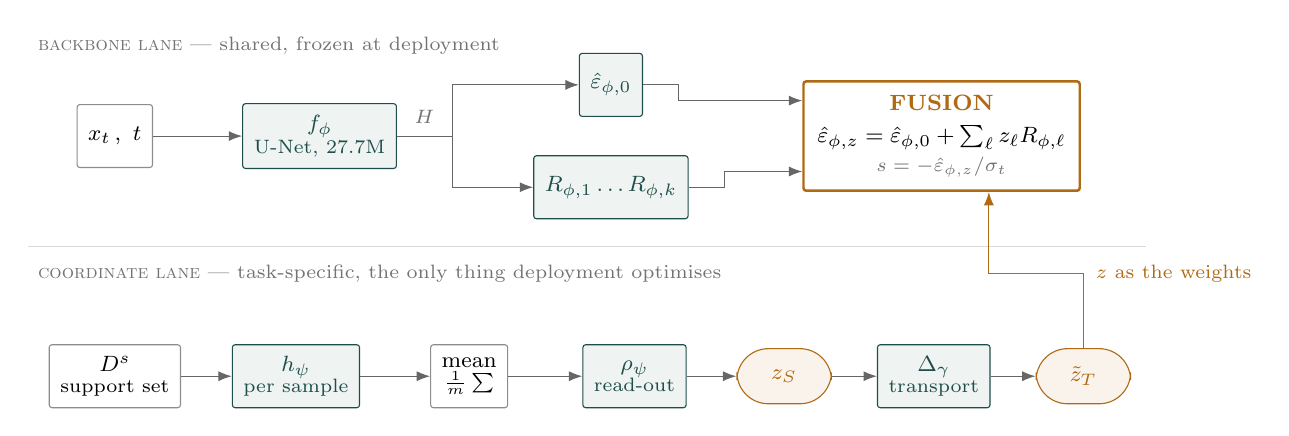
\begin{tikzpicture}[
  font=\footnotesize,
  bx/.style   ={draw=black!45, rounded corners=1pt, minimum height=8mm, inner sep=4pt, align=center},
  shd/.style  ={bx, draw=shared, fill=shared!7, text=shared},
  crd/.style  ={draw=coord, fill=coord!8, text=coord, rounded corners=4mm,
                minimum height=7mm, minimum width=12mm, align=center},
  fus/.style  ={draw=coord, line width=0.9pt, rounded corners=1pt, align=center, inner sep=5pt},
  ar/.style   ={-{Latex[length=1.7mm]}, black!60}
]
% ---------- backbone lane ----------
\node[black!55, anchor=west, font=\scriptsize] at (-0.2,3.05)
  {\textsc{backbone lane} --- shared, frozen at deployment};
\node[bx]  (in)   at (0.9,1.9)  {$x_t\,,\ t$};
\node[shd] (bb)   at (3.5,1.9)  {$f_\phi$\\[-1pt]\scriptsize U-Net, 27.7M};
\node[shd] (bh)   at (7.2,2.55) {$\epshat_{\phi,0}$};
\node[shd] (rh)   at (7.2,1.25) {$R_{\phi,1}\ldots R_{\phi,k}$};
\node[fus] (fu)   at (11.4,1.9)
  {\textcolor{coord}{\textbf{FUSION}}\\[2pt]
   $\epshat_{\phi,z}=\epshat_{\phi,0}+\sum_\ell z_\ell R_{\phi,\ell}$\\[1pt]
   \scriptsize\textcolor{black!55}{$s=-\epshat_{\phi,z}/\sigma_t$}};

\draw[ar] (in) -- (bb);
\draw[black!60] (bb.east) -- node[above=1pt, black!55, font=\scriptsize]{$H$} ++(0.7,0)
  coordinate (br);
\draw[ar] (br) |- (bh.west);
\draw[ar] (br) |- (rh.west);
\draw[ar] (bh.east) -- ++(0.45,0) |- ($(fu.west)+(0,0.45)$);
\draw[ar] (rh.east) -- ++(0.45,0) |- ($(fu.west)+(0,-0.45)$);

\draw[black!15] (-0.2,0.5) -- (14.0,0.5);

% ---------- coordinate lane ----------
\node[black!55, anchor=west, font=\scriptsize] at (-0.2,0.15)
  {\textsc{coordinate lane} --- task-specific, the only thing deployment optimises};
\node[bx]  (sup) at (0.9,-1.15) {$D^{s}$\\[-2pt]\scriptsize support set};
\node[shd] (hps) at (3.2,-1.15) {$h_\psi$\\[-2pt]\scriptsize per sample};
\node[bx]  (pool)at (5.4,-1.15) {mean\\[-2pt]\scriptsize $\frac{1}{m}\sum$};
\node[shd] (rps) at (7.5,-1.15) {$\rho_\psi$\\[-2pt]\scriptsize read-out};
\node[crd] (zs)  at (9.4,-1.15) {$\zS$};
\node[shd] (tp)  at (11.3,-1.15){$\Delta_\gamma$\\[-2pt]\scriptsize transport};
\node[crd] (zt)  at (13.2,-1.15){$\ztilT$};

\draw[ar] (sup) -- (hps);
\draw[ar] (hps) -- (pool);
\draw[ar] (pool) -- (rps);
\draw[ar] (rps) -- (zs);
\draw[ar] (zs) -- (tp);
\draw[ar] (tp) -- (zt);
\draw[-{Latex[length=1.7mm]}, coord] (zt.north) -- ++(0,0.95)
  node[right=1pt, coord, font=\scriptsize, anchor=west]{$z$ as the weights}
  -| ($(fu.south)+(0.6,0)$);
\end{tikzpicture}}


\caption{Architecture. Green marks the shared parameters $\phi$ and $\psi$, frozen at deployment;
amber marks the task coordinate, the only object deployment optimises---sixteen scalars against
27.8 million frozen weights. One pass of $f_\phi$ feeds both heads, which is what makes this one
network rather than $k$ separate denoisers. The transport map $\Delta_\gamma$ receives $\zS$ and
the relation descriptor only; no target sample reaches it, and that constraint is the proposition
under test.}
\label{fig:arch}
\end{figure}

\begin{table}[htbp]
\centering\small
\begin{tabular}{@{}llr p{7.0cm}@{}}
\toprule
\textbf{Symbol} & \textbf{Module} & \textbf{Params} & \textbf{Definition and constraint} \\
\midrule
$f_\phi$ & shared backbone & 27.74\,M
  & Maps $(x_t,t)$ to a feature tensor $H$ at input resolution. Carries no
    noise-prediction head of its own \\[2pt]
$\epshat_{\phi,0}$ & baseline head & 3{,}459
  & $1\times1$ convolution, $C_{\text{feat}}\!\to\!C_{\text{img}}$. The task-independent
    noise prediction \\[2pt]
$R_{\phi,1..k}$ & basis head & 55{,}344
  & Convolution to $k\,C_{\text{img}}$ channels, reshaped to $k$ image-shaped directions.
    Initialised small but non-zero \\[2pt]
$h_\psi,\ \rho_\psi$ & set encoder & 0.33\,M
  & Permutation-invariant map from a set to a coordinate. Source and target share this
    one encoder \\[2pt]
$\Delta_\gamma$ & transport map & 6{,}288
  & Residual multi-layer perceptron (MLP), $(k+d_c)\!\to\!64\!\to\!64\!\to\!k$, operating
    purely in coordinate space \\[2pt]
$z$ & \textbf{task coordinate} & \textbf{16}
  & The sole degree of freedom at deployment \\
\bottomrule
\end{tabular}
\caption{Module inventory at $k=16$, three image channels, $32\times32$ pixels. $\phi$ denotes
backbone and both heads; $\psi$ the encoder; $\gamma$ the transport map.}
\end{table}

% =========================================================================
\section{Dataset construction}
\label{sec:data}

CIFAR-100 is a two-level taxonomy: twenty superclasses, each holding exactly five fine classes,
each fine class holding exactly 600 images of $32\times32$ pixels in colour.

The split divides \textbf{semantic tasks, not images}. A fine class belongs entirely to one of the
three ways, and the division is made at the superclass level so that near-identical siblings
cannot straddle it.

\begin{figure}[htbp]
\centering
\resizebox{\textwidth}{!}{%
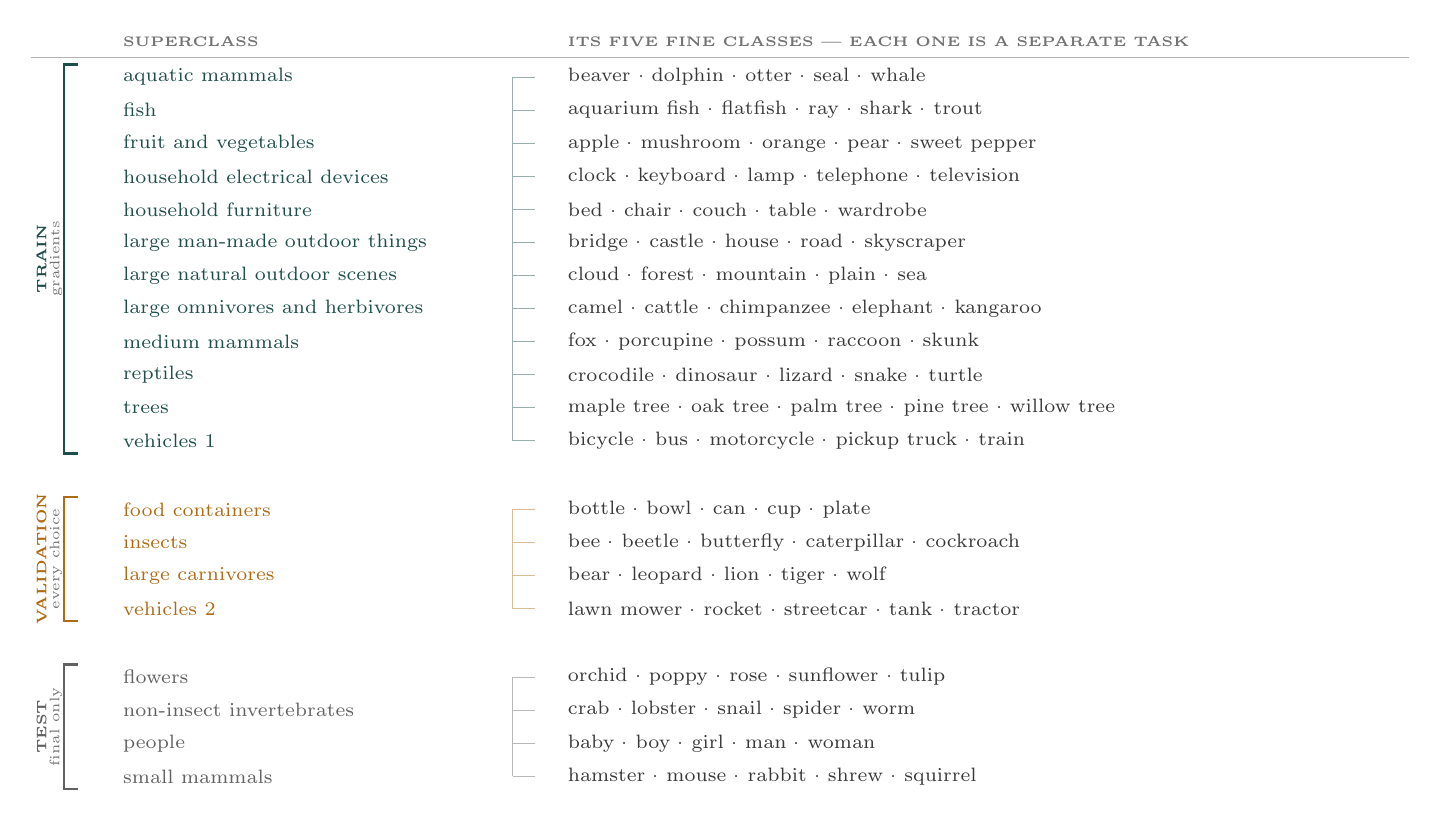
\begin{tikzpicture}[x=1cm, y=1cm]
% --- generated from the split file; see the header comment ---
\node[anchor=west, font=\tiny\bfseries, black!55] at (0.75,0.45) {SUPERCLASS};
\node[anchor=west, font=\tiny\bfseries, black!55] at (6.40,0.45) {ITS FIVE FINE CLASSES --- EACH ONE IS A SEPARATE TASK};
\draw[black!30, line width=.3pt] (-0.3,0.25) -- (17.2,0.25);
\draw[shared, line width=.8pt] (0.30,0.16) -- (0.12,0.16) -- (0.12,-4.78) -- (0.30,-4.78);
\node[rotate=90, font=\tiny\bfseries, shared] at (-0.16,-2.31) {TRAIN};
\node[rotate=90, font=\tiny, black!55] at (0.02,-2.31) {gradients};
\draw[shared, opacity=.45, line width=.3pt] (5.82,0.00) -- (5.82,-4.62);
\node[anchor=west, font=\scriptsize, shared] at (0.75,0.00) {aquatic mammals};
\draw[shared, opacity=.45, line width=.3pt] (5.82,0.00) -- (6.10,0.00);
\node[anchor=west, font=\scriptsize, black!78] at (6.40,0.00) {beaver \textperiodcentered\ dolphin \textperiodcentered\ otter \textperiodcentered\ seal \textperiodcentered\ whale};
\node[anchor=west, font=\scriptsize, shared] at (0.75,-0.42) {fish};
\draw[shared, opacity=.45, line width=.3pt] (5.82,-0.42) -- (6.10,-0.42);
\node[anchor=west, font=\scriptsize, black!78] at (6.40,-0.42) {aquarium fish \textperiodcentered\ flatfish \textperiodcentered\ ray \textperiodcentered\ shark \textperiodcentered\ trout};
\node[anchor=west, font=\scriptsize, shared] at (0.75,-0.84) {fruit and vegetables};
\draw[shared, opacity=.45, line width=.3pt] (5.82,-0.84) -- (6.10,-0.84);
\node[anchor=west, font=\scriptsize, black!78] at (6.40,-0.84) {apple \textperiodcentered\ mushroom \textperiodcentered\ orange \textperiodcentered\ pear \textperiodcentered\ sweet pepper};
\node[anchor=west, font=\scriptsize, shared] at (0.75,-1.26) {household electrical devices};
\draw[shared, opacity=.45, line width=.3pt] (5.82,-1.26) -- (6.10,-1.26);
\node[anchor=west, font=\scriptsize, black!78] at (6.40,-1.26) {clock \textperiodcentered\ keyboard \textperiodcentered\ lamp \textperiodcentered\ telephone \textperiodcentered\ television};
\node[anchor=west, font=\scriptsize, shared] at (0.75,-1.68) {household furniture};
\draw[shared, opacity=.45, line width=.3pt] (5.82,-1.68) -- (6.10,-1.68);
\node[anchor=west, font=\scriptsize, black!78] at (6.40,-1.68) {bed \textperiodcentered\ chair \textperiodcentered\ couch \textperiodcentered\ table \textperiodcentered\ wardrobe};
\node[anchor=west, font=\scriptsize, shared] at (0.75,-2.10) {large man-made outdoor things};
\draw[shared, opacity=.45, line width=.3pt] (5.82,-2.10) -- (6.10,-2.10);
\node[anchor=west, font=\scriptsize, black!78] at (6.40,-2.10) {bridge \textperiodcentered\ castle \textperiodcentered\ house \textperiodcentered\ road \textperiodcentered\ skyscraper};
\node[anchor=west, font=\scriptsize, shared] at (0.75,-2.52) {large natural outdoor scenes};
\draw[shared, opacity=.45, line width=.3pt] (5.82,-2.52) -- (6.10,-2.52);
\node[anchor=west, font=\scriptsize, black!78] at (6.40,-2.52) {cloud \textperiodcentered\ forest \textperiodcentered\ mountain \textperiodcentered\ plain \textperiodcentered\ sea};
\node[anchor=west, font=\scriptsize, shared] at (0.75,-2.94) {large omnivores and herbivores};
\draw[shared, opacity=.45, line width=.3pt] (5.82,-2.94) -- (6.10,-2.94);
\node[anchor=west, font=\scriptsize, black!78] at (6.40,-2.94) {camel \textperiodcentered\ cattle \textperiodcentered\ chimpanzee \textperiodcentered\ elephant \textperiodcentered\ kangaroo};
\node[anchor=west, font=\scriptsize, shared] at (0.75,-3.36) {medium mammals};
\draw[shared, opacity=.45, line width=.3pt] (5.82,-3.36) -- (6.10,-3.36);
\node[anchor=west, font=\scriptsize, black!78] at (6.40,-3.36) {fox \textperiodcentered\ porcupine \textperiodcentered\ possum \textperiodcentered\ raccoon \textperiodcentered\ skunk};
\node[anchor=west, font=\scriptsize, shared] at (0.75,-3.78) {reptiles};
\draw[shared, opacity=.45, line width=.3pt] (5.82,-3.78) -- (6.10,-3.78);
\node[anchor=west, font=\scriptsize, black!78] at (6.40,-3.78) {crocodile \textperiodcentered\ dinosaur \textperiodcentered\ lizard \textperiodcentered\ snake \textperiodcentered\ turtle};
\node[anchor=west, font=\scriptsize, shared] at (0.75,-4.20) {trees};
\draw[shared, opacity=.45, line width=.3pt] (5.82,-4.20) -- (6.10,-4.20);
\node[anchor=west, font=\scriptsize, black!78] at (6.40,-4.20) {maple tree \textperiodcentered\ oak tree \textperiodcentered\ palm tree \textperiodcentered\ pine tree \textperiodcentered\ willow tree};
\node[anchor=west, font=\scriptsize, shared] at (0.75,-4.62) {vehicles 1};
\draw[shared, opacity=.45, line width=.3pt] (5.82,-4.62) -- (6.10,-4.62);
\node[anchor=west, font=\scriptsize, black!78] at (6.40,-4.62) {bicycle \textperiodcentered\ bus \textperiodcentered\ motorcycle \textperiodcentered\ pickup truck \textperiodcentered\ train};
\draw[coord, line width=.8pt] (0.30,-5.33) -- (0.12,-5.33) -- (0.12,-6.91) -- (0.30,-6.91);
\node[rotate=90, font=\tiny\bfseries, coord] at (-0.16,-6.12) {VALIDATION};
\node[rotate=90, font=\tiny, black!55] at (0.02,-6.12) {every choice};
\draw[coord, opacity=.45, line width=.3pt] (5.82,-5.49) -- (5.82,-6.75);
\node[anchor=west, font=\scriptsize, coord] at (0.75,-5.49) {food containers};
\draw[coord, opacity=.45, line width=.3pt] (5.82,-5.49) -- (6.10,-5.49);
\node[anchor=west, font=\scriptsize, black!78] at (6.40,-5.49) {bottle \textperiodcentered\ bowl \textperiodcentered\ can \textperiodcentered\ cup \textperiodcentered\ plate};
\node[anchor=west, font=\scriptsize, coord] at (0.75,-5.91) {insects};
\draw[coord, opacity=.45, line width=.3pt] (5.82,-5.91) -- (6.10,-5.91);
\node[anchor=west, font=\scriptsize, black!78] at (6.40,-5.91) {bee \textperiodcentered\ beetle \textperiodcentered\ butterfly \textperiodcentered\ caterpillar \textperiodcentered\ cockroach};
\node[anchor=west, font=\scriptsize, coord] at (0.75,-6.33) {large carnivores};
\draw[coord, opacity=.45, line width=.3pt] (5.82,-6.33) -- (6.10,-6.33);
\node[anchor=west, font=\scriptsize, black!78] at (6.40,-6.33) {bear \textperiodcentered\ leopard \textperiodcentered\ lion \textperiodcentered\ tiger \textperiodcentered\ wolf};
\node[anchor=west, font=\scriptsize, coord] at (0.75,-6.75) {vehicles 2};
\draw[coord, opacity=.45, line width=.3pt] (5.82,-6.75) -- (6.10,-6.75);
\node[anchor=west, font=\scriptsize, black!78] at (6.40,-6.75) {lawn mower \textperiodcentered\ rocket \textperiodcentered\ streetcar \textperiodcentered\ tank \textperiodcentered\ tractor};
\draw[black!62, line width=.8pt] (0.30,-7.46) -- (0.12,-7.46) -- (0.12,-9.04) -- (0.30,-9.04);
\node[rotate=90, font=\tiny\bfseries, black!62] at (-0.16,-8.25) {TEST};
\node[rotate=90, font=\tiny, black!55] at (0.02,-8.25) {final only};
\draw[black!62, opacity=.45, line width=.3pt] (5.82,-7.62) -- (5.82,-8.88);
\node[anchor=west, font=\scriptsize, black!62] at (0.75,-7.62) {flowers};
\draw[black!62, opacity=.45, line width=.3pt] (5.82,-7.62) -- (6.10,-7.62);
\node[anchor=west, font=\scriptsize, black!78] at (6.40,-7.62) {orchid \textperiodcentered\ poppy \textperiodcentered\ rose \textperiodcentered\ sunflower \textperiodcentered\ tulip};
\node[anchor=west, font=\scriptsize, black!62] at (0.75,-8.04) {non-insect invertebrates};
\draw[black!62, opacity=.45, line width=.3pt] (5.82,-8.04) -- (6.10,-8.04);
\node[anchor=west, font=\scriptsize, black!78] at (6.40,-8.04) {crab \textperiodcentered\ lobster \textperiodcentered\ snail \textperiodcentered\ spider \textperiodcentered\ worm};
\node[anchor=west, font=\scriptsize, black!62] at (0.75,-8.46) {people};
\draw[black!62, opacity=.45, line width=.3pt] (5.82,-8.46) -- (6.10,-8.46);
\node[anchor=west, font=\scriptsize, black!78] at (6.40,-8.46) {baby \textperiodcentered\ boy \textperiodcentered\ girl \textperiodcentered\ man \textperiodcentered\ woman};
\node[anchor=west, font=\scriptsize, black!62] at (0.75,-8.88) {small mammals};
\draw[black!62, opacity=.45, line width=.3pt] (5.82,-8.88) -- (6.10,-8.88);
\node[anchor=west, font=\scriptsize, black!78] at (6.40,-8.88) {hamster \textperiodcentered\ mouse \textperiodcentered\ rabbit \textperiodcentered\ shrew \textperiodcentered\ squirrel};
\end{tikzpicture}}
\caption{The three-way split in full. Twelve superclasses and their sixty fine classes train the
model; four superclasses and twenty fine classes carry every hyperparameter choice; four
superclasses and twenty fine classes are reserved for the final number. Splitting by superclass
rather than by fine class keeps near-identical siblings such as maple and oak on the same side:
the test set contains no close relative of anything seen in training.}
\label{fig:split}
\end{figure}

\subsection{Within one fine class}

Each class's 600 images are shuffled once by a seed-derived permutation and cut into two disjoint
pools, then each pool is cut again into support and query.

\begin{table}[htbp]
\centering\small
\begin{tabular}{@{}llrl p{5.2cm}@{}}
\toprule
\textbf{Stream} & \textbf{Symbol} & \textbf{Images} & \textbf{Pixels} & \textbf{Drawn per episode} \\
\midrule
source support & $\Dss$ & 300 & clean       & $\MS$ sampled without replacement \\
source query   & $\Dqs$ & 50  & clean       & 32 sampled without replacement \\
target support & $\Dst$ & 20 reserved & transformed & the first $\KT$, so support sets are
                                                       nested in $\KT$ \\
target query   & $\Dqt$ & 230 & transformed & 32 sampled without replacement \\
\bottomrule
\end{tabular}
\caption{Source pool 350 images, target pool 250, verified pairwise disjoint by global image
identifier: 600 identifiers, 600 unique. Source and target therefore use \emph{different
underlying images}---pairing a clean image with its own transformed copy would leak, and real
domain shift does not arrive in matched pairs.}
\end{table}

\subsection{How the target domain is made}

The target domain is produced by applying a fixed, deterministic, semantics-preserving image
transformation to the target pool. Three are implemented, in the style of the CIFAR-100-C
benchmark, each at five severities; severity~3 is the default.

\begin{table}[htbp]
\centering\footnotesize
\begin{tabular}{@{}llll@{}}
\toprule
\textbf{Transformation} & \textbf{Operation} & \textbf{Parameter, severity 1\,\ldots\,5} & \textbf{mean $|\Delta$px$|$} \\
\midrule
Gaussian blur     & separable Gaussian convolution     & $\sigma=0.5,\,0.75,\,1.0,\,1.5,\,2.0$ & 0.085 \\
Additive noise    & seeded per image identifier        & $\mathrm{std}=0.08,\,0.12,\,0.18,\,0.26,\,0.38$ & 0.133 \\
Contrast          & shrink toward each image's own mean & factor $=0.75,\,0.6,\,0.45,\,0.3,\,0.2$ & 0.184 \\
\bottomrule
\end{tabular}
\caption{Change measured on the $[-1,1]$ pixel scale at severity 3. Every transformation is
reproducible from the triple (image identifier, type, severity); the additive-noise transformation
derives its random seed from the image identifier, without which the ``same'' target domain would
differ between runs.}
\end{table}

% =========================================================================
\section{Data flow}
\label{sec:flow}

Support sets flow into the encoder and produce coordinates. Query sets flow into the diffusion
forward process and produce losses. No stream does both.

\paragraph{Two operations, easily conflated.}
One of the three transformations is itself called Gaussian noise, so the two are kept apart
throughout this document:

\begin{itemize}[leftmargin=*, itemsep=2pt]
\item the \textbf{image transformation}---blur, additive noise or contrast reduction---applied
      when a target-stream image is fetched. It defines \emph{what the target domain is}, and the
      model must learn to generate images that carry it;
\item the \textbf{diffusion forward process} $x_t=\alpha_t x_0+\sigma_t\varepsilon$, applied to
      query batches during training. It is part of the \emph{training mechanism} and applies
      equally to source and target.
\end{itemize}

\begin{table}[htbp]
\centering\small
\begin{tabular}{@{}lccp{6.4cm}@{}}
\toprule
\textbf{Stream} & \textbf{transformation} & \textbf{forward process} & \textbf{Why} \\
 & \scriptsize defines the target domain & \scriptsize the training mechanism & \\
\midrule
$\Dss$ & no  & no  & source domain, and support sets only produce coordinates \\
$\Dqs$ & no  & \textbf{yes} & source domain, but a query set carries a denoising loss \\
$\Dst$ & \textbf{yes} & no  & target domain, but a support set only produces a coordinate \\
$\Dqt$ & \textbf{yes} & \textbf{yes} & target domain and a query set: both apply \\
\bottomrule
\end{tabular}
\caption{Read down the first column for ``which domain is this'', and down the second for ``does
this stream carry a loss''. The two questions are independent, which is why the answer is a
$2\times2$ rather than a single split.}
\end{table}

\begin{figure}[htbp]
\centering
\resizebox{\textwidth}{!}{%
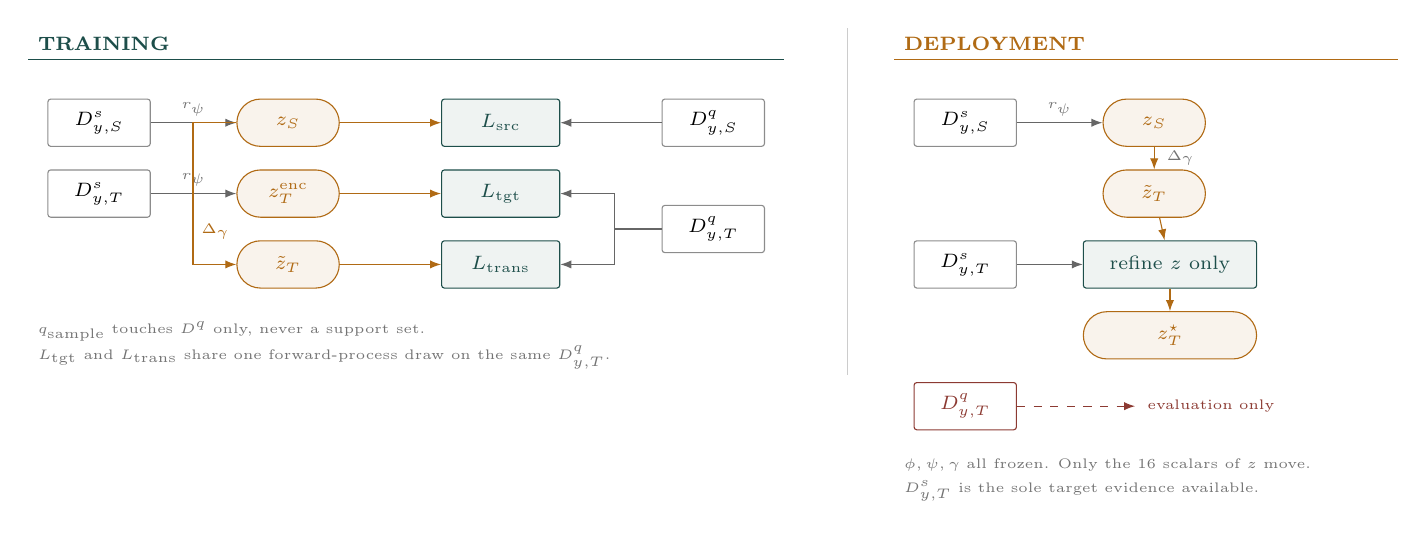
\begin{tikzpicture}[
  font=\scriptsize,
  bx/.style ={draw=black!45, rounded corners=1pt, minimum height=6mm, minimum width=13mm,
              inner sep=2pt, align=center},
  shd/.style={bx, draw=shared, fill=shared!7, text=shared, minimum width=15mm},
  crd/.style={draw=coord, fill=coord!8, text=coord, rounded corners=3mm,
              minimum height=6mm, minimum width=13mm, align=center},
  ar/.style ={-{Latex[length=1.4mm]}, black!60},
  arc/.style={-{Latex[length=1.4mm]}, coord},
  aro/.style={-{Latex[length=1.4mm]}, overturn, dashed}
]
% =============== training ===============
\node[shared, anchor=west, font=\scriptsize\bfseries] at (0,4.0) {TRAINING};
\draw[shared] (0,3.8) -- (9.6,3.8);

% supports, coordinates, losses and queries occupy four columns; each loss sits on
% the same row as the coordinate that feeds it, so no arrow needs to cross another
\node[bx]  (ss) at (0.9,3.0)  {$\Dss$};
\node[bx]  (ts) at (0.9,2.1)  {$\Dst$};
\node[crd] (zs) at (3.3,3.0)  {$\zS$};
\node[crd] (ze) at (3.3,2.1)  {$\zencT$};
\node[crd] (zt) at (3.3,1.2)  {$\ztilT$};
\node[shd] (ls) at (6.0,3.0)  {$L_{\mathrm{src}}$};
\node[shd] (lt) at (6.0,2.1)  {$L_{\mathrm{tgt}}$};
\node[shd] (lr) at (6.0,1.2)  {$L_{\mathrm{trans}}$};
\node[bx]  (qs) at (8.7,3.0)  {$\Dqs$};
\node[bx]  (qt) at (8.7,1.65) {$\Dqt$};

\draw[ar] (ss) -- node[above=-1pt, font=\tiny, black!55]{$r_\psi$} (zs);
\draw[ar] (ts) -- node[above=-1pt, font=\tiny, black!55]{$r_\psi$} (ze);

% z_S to z-tilde, routed clear of every box on a lane of its own
\draw[arc] (zs.west) -- ++(-0.55,0) |- (zt.west);
\node[coord, font=\tiny, anchor=east] at (2.68,1.62) {$\Delta_\gamma$};

\draw[arc] (zs) -- (ls);
\draw[arc] (ze) -- (lt);
\draw[arc] (zt) -- (lr);

\draw[ar] (qs) -- (ls);
\draw[ar] (qt.west) -- ++(-0.6,0) |- (lt.east);
\draw[ar] (qt.west) -- ++(-0.6,0) |- (lr.east);

\node[anchor=west, black!55, font=\tiny] at (0,0.35)
  {$q_{\text{sample}}$ touches $D^{q}$ only, never a support set.};
\node[anchor=west, black!55, font=\tiny] at (0,0.02)
  {$L_{\mathrm{tgt}}$ and $L_{\mathrm{trans}}$ share one forward-process draw on the same $\Dqt$.};

% =============== deployment ===============
\draw[black!20] (10.4,-0.2) -- (10.4,4.2);
\node[coord, anchor=west, font=\scriptsize\bfseries] at (11.0,4.0) {DEPLOYMENT};
\draw[coord] (11.0,3.8) -- (17.4,3.8);

\node[bx]  (ss2) at (11.9,3.0) {$\Dss$};
\node[crd] (zs2) at (14.3,3.0) {$\zS$};
\node[crd] (zt2) at (14.3,2.1) {$\ztilT$};
\node[bx]  (ts2) at (11.9,1.2) {$\Dst$};
\node[shd, minimum width=22mm] (rf) at (14.5,1.2) {refine $z$ only};
\node[crd, minimum width=22mm] (zst) at (14.5,0.3) {$\zstarT$};
\node[bx, draw=overturn, text=overturn] (qt2) at (11.9,-0.6) {$\Dqt$};

\draw[ar]  (ss2) -- node[above=-1pt, font=\tiny, black!55]{$r_\psi$} (zs2);
\draw[arc] (zs2) -- node[right=1pt, font=\tiny, black!55]{$\Delta_\gamma$} (zt2);
\draw[arc] (zt2) -- (rf);
\draw[ar]  (ts2) -- (rf);
\draw[arc] (rf)  -- (zst);
\draw[aro] (qt2.east) -- ++(1.5,0)
  node[right=1pt, overturn, font=\tiny, anchor=west]{evaluation only};

\node[anchor=west, black!55, font=\tiny] at (11.0,-1.35)
  {$\phi,\psi,\gamma$ all frozen. Only the 16 scalars of $z$ move.};
\node[anchor=west, black!55, font=\tiny] at (11.0,-1.68)
  {$\Dst$ is the sole target evidence available.};
\end{tikzpicture}}

\caption{Where each stream goes. The structural difference between the two halves is which arrows
exist: training computes three losses and every module receives gradient; deployment freezes all
parameters and refines the coordinate alone. The dashed path is the protocol's red line---target
query data reaches evaluation and nothing else, enforced at the type level, since the refinement
function has no parameter through which it could arrive.}
\label{fig:flow}
\end{figure}

% =========================================================================
\section{Loss functions}
\label{sec:loss}

\subsection{Notation}

Write $y$ for a semantic task, $t\sim\mathcal{U}\{0,\dots,T-1\}$ for a diffusion timestep and
$\varepsilon\sim\mathcal{N}(0,I)$ for the noise. The forward process is
\begin{equation}
x_t \;=\; \alpha_t\,x_0 \;+\; \sigma_t\,\varepsilon,
\qquad \alpha_t^{2}+\sigma_t^{2}=1,
\end{equation}
and the weighting $w(t)=1$ throughout---the plain $\varepsilon$-prediction objective.

\subsection{The three coordinates}

\begin{align}
\zS      &= \rho_\psi\!\left( \frac{1}{|\Dss|}\sum_{x\in \Dss} h_\psi(x) \right) \\
\zencT   &= \rho_\psi\!\left( \frac{1}{|\Dst|}\sum_{x\in \Dst} h_\psi(x) \right) \\
\ztilT   &= \zS + \Delta_\gamma\!\left( \zS,\, c_{S\to T} \right)
\end{align}

The third line takes $\zS$ and the relation descriptor and nothing else. It contains no target
sample.

\subsection{The predictor each loss is built on}

Every term below evaluates the same predictor at a different coordinate:
\begin{equation}
\epshat_{\phi,z}(x_t,t) \;=\; \epshat_{\phi,0}(x_t,t)
  \;+\; \sum_{\ell=1}^{k} z_\ell \, R_{\phi,\ell}(x_t,t)
\label{eq:pred}
\end{equation}

\subsection{Term 1 --- source denoising loss}

Trains the backbone and the baseline head on the source domain, and is the only signal that shapes
$\zS$ through the encoder.
\begin{equation}
L_{\mathrm{src}} \;=\;
\mathop{\mathbb{E}}_{x_0\sim \Dqs}\ \mathop{\mathbb{E}}_{t}\ \mathop{\mathbb{E}}_{\varepsilon}
\Big[\, w(t)\, \big\| \varepsilon - \epshat_{\phi,\zS}(\alpha_t x_0+\sigma_t\varepsilon,\, t) \big\|_2^2 \,\Big]
\end{equation}

\subsection{Term 2 --- target denoising loss, encoder coordinate}

The same functional on target-domain query images, using the coordinate encoded from the $\KT$
target support images. This is what teaches the encoder to produce meaningful coordinates for a
target set; without it the coordinate space would be shaped by source data alone.
\begin{equation}
L_{\mathrm{tgt}} \;=\;
\mathop{\mathbb{E}}_{x_0\sim \Dqt}\ \mathop{\mathbb{E}}_{t}\ \mathop{\mathbb{E}}_{\varepsilon}
\Big[\, w(t)\, \big\| \varepsilon - \epshat_{\phi,\zencT}(\alpha_t x_0+\sigma_t\varepsilon,\, t) \big\|_2^2 \,\Big]
\end{equation}

\subsection{Term 3 --- transport denoising loss}

Identical to term 2 but for the coordinate: the transported one, predicted from source data alone.
This is the only term that trains $\Delta_\gamma$.
\begin{equation}
L_{\mathrm{trans}} \;=\;
\mathop{\mathbb{E}}_{x_0\sim \Dqt}\ \mathop{\mathbb{E}}_{t}\ \mathop{\mathbb{E}}_{\varepsilon}
\Big[\, w(t)\, \big\| \varepsilon - \epshat_{\phi,\ztilT}(\alpha_t x_0+\sigma_t\varepsilon,\, t) \big\|_2^2 \,\Big]
\end{equation}

\subsection{Term 4 --- coordinate regulariser}

A light penalty preventing the encoder from drifting to coordinates of large magnitude. Set too
weakly, the encoder may emit a near-constant vector of substantial size, turning the basis into
extra shared capacity; set too strongly, the coordinate loses its influence.
\begin{equation}
L_{z} \;=\; \|\zS\|_2^2 \;+\; \|\zencT\|_2^2
\end{equation}
Note that $\ztilT$ is absent, since penalising it would penalise $\Delta_\gamma$ for moving.

\subsection{The total}

\begin{equation}
\boxed{\;
L_{\mathrm{meta}} \;=\; L_{\mathrm{src}}
  \;+\; \lambda_{T}\,L_{\mathrm{tgt}}
  \;+\; \lambda_{\mathrm{tr}}\,L_{\mathrm{trans}}
  \;+\; \lambda_{z}\,L_{z} \;}
\qquad \lambda_{T}=\lambda_{\mathrm{tr}}=1,\quad \lambda_{z}=10^{-4}
\end{equation}

\subsection{What is actually computed each step}

The expectations above are estimated by a single Monte-Carlo draw per query image. With a batch of
$B=32$ query images, one timestep and one noise vector drawn independently per image, and
$C\!\cdot\!H\!\cdot\!W = 3\cdot32\cdot32$ pixels:
\begin{align}
t_i &\sim \mathcal{U}\{0,\dots,999\}, \qquad
\varepsilon_i \sim \mathcal{N}(0,I), \qquad
x_{i,t} = \alpha_{t_i} x_i + \sigma_{t_i}\varepsilon_i \\[4pt]
\widehat{L}(D,z) &= \frac{1}{B}\sum_{i=1}^{B} w(t_i)\;
  \left[\, \frac{1}{C H W}\sum_{\text{pixels}}
  \big( \varepsilon_i - \epshat_{\phi,z}(x_{i,t},t_i) \big)^2 \right]
\end{align}

Two details matter for reproduction. The inner reduction is a \textbf{mean over pixels, not a
sum}, so the loss scale is independent of image resolution. And $w(t)=1$ throughout;
signal-to-noise and truncated signal-to-noise weightings are implemented but were not used in any
experiment reported here.

\paragraph{Terms 2 and 3 share their random draws.}
One batch $\{x_0\}$, one set of timesteps $\{t_i\}$, one set of noise vectors
$\{\varepsilon_i\}$, and one backbone pass serve both. Their difference is therefore a paired
estimate of what the transport map adds over encoding the target directly, with the sampling noise
common to both cancelling out.

\subsection{The deployment objective}

At deployment $\phi,\psi,\gamma$ are frozen and a single coordinate is fitted on the $\KT$ target
support images:
\begin{equation}
\zstarT \;=\; \arg\min_{z} \left\{
  \frac{1}{\KT}\sum_{i=1}^{\KT}
  \mathop{\mathbb{E}}_{t,\varepsilon}\Big[\, w(t)\,\big\| \varepsilon
    - \epshat_{\phi,z}(x^{T}_{i,t},t) \big\|_2^2 \,\Big]
  \;+\; \frac{\beta_0}{\KT}\,\big\| z - \ztilT \big\|_2^2
\right\}
\label{eq:refine}
\end{equation}
with $J=25$ steps, $\eta_z=10^{-2}$, $\beta_0=1$, and 16 $(t,\varepsilon)$ draws per step.

Both divisions by $\KT$ matter. Dividing the denoising term holds the gradient scale steady across
support sizes; dividing the prior term by the same quantity makes the source-derived prior's
relative influence decay as target evidence accumulates---it dominates at one sample and recedes
once samples are plentiful.

% =========================================================================
\section{Experiments run}
\label{sec:experiments}

\subsection{What the numbers in these tables are}

Seven quantities appear across the tables below. Two exist only on Gaussian mixtures, where the
true score function is available in closed form; the rest apply to the image experiments as well.

\begin{table}[htbp]
\centering\small
\begin{tabular}{@{}p{3.1cm}p{6.3cm}p{4.6cm}@{}}
\toprule
\textbf{Quantity} & \textbf{Definition} & \textbf{Units, and which way is better} \\
\midrule
relative score-field error
  & $\sqrt{\sum\|\hat{s}-s^{\star}\|^2 \big/ \sum\|s^{\star}\|^2}$, accumulated over five
    timesteps at 2048 points each, drawn from the true noised distribution $x_t\sim p_t$ rather
    than a uniform grid
  & dimensionless; 0 is exact, 1 is as wrong as predicting zero. Lower is better \\[2pt]
sliced Wasserstein-2
  & Project both point clouds onto 256 random unit directions, sort, take the root-mean-square
    difference
  & data units. Lower is better \\[2pt]
denoising loss
  & $\mathbb{E}[w(t)\|\varepsilon-\epshat\|^2]$ on held-out target query images. The training
    objective itself, on data never fitted
  & squared-noise units; typical converged values 0.02--0.15. Lower is better \\[2pt]
gain vs $z=0$
  & $\text{loss}(z{=}0)-\text{loss}(\text{correct }z)$
  & same units as the loss. Higher \emph{looks} better---see E9 \\[2pt]
basis usage $r_{\text{basis}}$
  & $\|\sum_\ell z_\ell R_\ell\| / (\|\epshat_0\|+\epsilon)$, per sample
  & dimensionless; 0 means the basis is unused \\[2pt]
coordinate spread
  & mean pairwise distance between episode coordinates, divided by their mean norm
  & dimensionless; below 0.05 the encoder emits a near-constant \\[2pt]
relative coordinate distance
  & $\|z-z^{\text{abund}}_T\| / \|z^{\text{abund}}_T\|$, reference encoded from 230 target images
  & dimensionless. Lower is better \\
\bottomrule
\end{tabular}
\end{table}

Every $\pm$ figure is a 95\% confidence interval on a \textbf{paired per-episode difference}, not a
standard deviation across runs: both strategies are evaluated on the same episode with the same
noise draw, the difference taken per episode, and the interval formed over episodes. Between-task
variance is roughly an order of magnitude larger than the effects being measured, so an unpaired
comparison over a handful of episodes returns an arbitrary sign.

\subsection{E1 --- analytic validation on two-dimensional Gaussian mixtures}

\textit{$k=16$, 80{,}000 steps, 12 unseen tasks. Mechanism validated.}

\paragraph{Procedure.} Each task is a four-component Gaussian mixture; the target is that mixture
under a controlled relation (rotation, translation, covariance scaling, reweighting) that recurs
across tasks. Gaussian noising preserves the mixture form, so the true score has a closed form and
model output is compared against \emph{truth} rather than sample plausibility. The backbone is a
1.3\,M-parameter residual MLP; every other module and the entire training loop are unchanged from
the image path.

\begin{table}[htbp]
\centering\small
\begin{tabular}{@{}lrrrrrr@{}}
\toprule
& \multicolumn{2}{c}{$\KT=1$} & \multicolumn{2}{c}{$\KT=5$} & \multicolumn{2}{c}{$\KT=20$} \\
\cmidrule(lr){2-3}\cmidrule(lr){4-5}\cmidrule(lr){6-7}
\textbf{Strategy} & score err & SW$_2$ & score err & SW$_2$ & score err & SW$_2$ \\
\midrule
no adaptation ($z=0$)     & 0.9045 & 0.9726 & 0.9049 & 0.9879 & 0.9055 & 0.9802 \\
target only               & 1.0478 & 0.8966 & 0.8393 & 0.6595 & 0.7086 & 0.5336 \\
reuse $\zS$               & 0.8243 & 0.7465 & 0.8010 & 0.6240 & 0.7586 & 0.6608 \\
transport, no refine      & 0.8060 & 0.7216 & 0.8028 & 0.7233 & 0.8103 & 0.7046 \\
\textbf{transport + refine} & \textbf{0.7787} & \textbf{0.6951} & \textbf{0.7547} & \textbf{0.6717} & \textbf{0.7160} & \textbf{0.6117} \\
full fine-tuning, $J=25$  & 0.9169 & 0.8991 & 0.8591 & 0.6864 & 0.8330 & 0.5767 \\
full fine-tuning, $J=2000$& 6.9697 & 1.5356 & 5.3606 & 0.7293 & 1.5218 & 0.3942 \\
abundant-target oracle    & 0.6614 & 0.5561 & 0.6632 & 0.5289 & 0.6640 & 0.5203 \\
\bottomrule
\end{tabular}
\caption{Relative score-field error and sliced Wasserstein-2 distance. Both lower-is-better.}
\end{table}

\begin{table}[htbp]
\centering\small
\begin{tabular}{@{}lrrr@{}}
\toprule
& \multicolumn{3}{c}{paired difference in relative score-field error} \\
\cmidrule(lr){2-4}
\textbf{Transport minus\ldots} & $\KT=1$ & $\KT=5$ & $\KT=20$ \\
\midrule
no adaptation              & $+0.1529\pm0.0273$ & $+0.1913\pm0.0221$ & $+0.2263\pm0.0217$ \\
target only                & $+0.2397\pm0.0338$ & $+0.0861\pm0.0210$ & $+0.0015\pm0.0106$ \\
reuse $\zS$                & $+0.0859\pm0.0287$ & $+0.0611\pm0.0214$ & $+0.0626\pm0.0196$ \\
transport without refinement & $+0.0078\pm0.0072$ & $+0.0473\pm0.0136$ & $+0.0831\pm0.0130$ \\
\bottomrule
\end{tabular}
\caption{32 unseen tasks $\times$ 3 seeds, paired. Every interval excludes zero except transport
against target-only at $\KT=20$, where the advantage has correctly vanished. The margin being
largest at one sample and gone by twenty is the shape the method predicts, and this is the
strongest positive evidence in the programme.}
\end{table}

\subsection{E2 --- CIFAR-100, sibling fine classes}

\textit{$k=16$, 6{,}000 steps, stopped early. Coordinate collapsed.}

\paragraph{Procedure.} Source and target are two \emph{different} fine classes of one
superclass---beaver and dolphin, say. Since CIFAR-100 is balanced, the target's scarcity is imposed
by restricting its support set rather than inherited from the data.

\paragraph{Result.} The coordinate collapses to a near-constant: relative spread across episodes
stays at 0.013--0.026 against a 0.05 threshold, flat over six diagnostic points while the denoising
loss plateaued. Dissecting the step-5000 checkpoint located the cause: pooled encoder features have
a cross-episode spread of only 0.058, and the source-to-target distance (0.067) is indistinguishable
from it---one flower species reads much like another. Adding second-moment pooling did not fix it.
Retained as a low-relatedness stress test.

\subsection{E3 --- CIFAR-100, one fixed transformation}

\textit{$k=16$, 50{,}000 steps, Gaussian blur at severity 3. Benefit decays to zero.}

\paragraph{Procedure.} The main protocol: source is a class's clean images, target is different
images of the same class under Gaussian blur. Diagnostics every 1000 steps on held-out classes.

\paragraph{Result.} Collapse is solved---coordinate spread rises to 0.32 and source is cleanly
separated from target (1.45). But the benefit vanishes over training:

\begin{center}\small
\begin{tabular}{@{}lrrrrrr@{}}
\toprule
step & 1000 & 2000 & 5000 & 10000 & 20000 & 50000 \\
\midrule
gain vs $z=0$ & 0.083 & 0.084 & 0.058 & 0.019 & 0.001 & 0.0002 \\
basis usage   & 0.254 & 0.402 & 0.317 & 0.161 & 0.032 & 0.012 \\
\bottomrule
\end{tabular}
\end{center}

Two quantities move in opposite directions: the encoder keeps improving while the basis is
progressively abandoned.

\subsection{E4 --- CIFAR-100, three transformations}

\textit{$k=16$, 50{,}000 steps, blur, additive noise and contrast. Same decay.}

\paragraph{Procedure.} Identical to E3 except that each episode draws one of three transformations,
so the relation descriptor is active and the backbone cannot know which target domain applies
without the coordinate. The relation is indexed by transformation type, which is legitimate because
transformations recur across all three splits.

\paragraph{Result.} The hypothesis failed. Gain peaks at 0.078 and decays to 0.0016; basis usage
$0.29\to0.039$; coordinate spread meanwhile climbs to 1.21.

\begin{table}[htbp]
\centering\small
\begin{tabular}{@{}lrrr@{}}
\toprule
& \multicolumn{3}{c}{denoising loss on held-out target query, lower is better} \\
\cmidrule(lr){2-4}
\textbf{Strategy} & $\KT=1$ & $\KT=5$ & $\KT=20$ \\
\midrule
no adaptation ($z=0$)  & 0.0902 & 0.0902 & 0.0902 \\
target support only    & 0.0888 & 0.0887 & 0.0887 \\
reuse $\zS$            & 0.0901 & 0.0890 & 0.0888 \\
transport, no refine   & 0.0887 & 0.0887 & 0.0887 \\
\textbf{transport + refine} & \textbf{0.0887} & \textbf{0.0887} & \textbf{0.0887} \\
oracle (fits on target query) & 0.0887 & 0.0887 & 0.0887 \\
\bottomrule
\end{tabular}
\caption{Any non-zero coordinate beats $z=0$ by $0.0015\pm0.0002$---statistically real, 1.7\% of
the loss. No coordinate beats any other: transport, refinement and even the oracle upper bound land
on the same number, and $\KT$ changes nothing.}
\end{table}

\subsection{E5 --- coordinate dimension sweep}

\textit{$k\in\{16,32,64\}$, 20{,}000 steps each, validation classes. $k$ is not the bottleneck.}

\paragraph{Procedure.} Three separate training runs, identical but for $k$, which changes the basis
head's output channel count and therefore requires retraining.

\begin{table}[htbp]
\centering\small
\begin{tabular}{@{}rrrrr@{}}
\toprule
& \multicolumn{2}{c}{gain vs $z=0$ at its peak} & gain vs $z=0$ & basis usage \\
\cmidrule(lr){2-3}
$k$ & value & step & at 20k steps & at 20k steps \\
\midrule
16 & 0.0839 & 2000 & 0.0007 & 0.0286 \\
32 & 0.1050 & 1000 & 0.0005 & 0.0244 \\
64 & 0.1288 & 1000 & 0.0004 & 0.0203 \\
\bottomrule
\end{tabular}
\caption{Quadrupling the coordinate dimension changes nothing at convergence. A larger $k$ raises
the early peak and then decays slightly further.}
\end{table}

\subsection{E6 --- backbone capacity sweep}

\textit{$k=32$ fixed, base channels $\in\{128,64,32\}$, 20{,}000 steps. Read as success; later
overturned.}

\paragraph{Procedure.} Coordinate dimension held at 32 while the backbone shrinks. The 64-channel
run differs from the 128 only in width---same depth, same attention---so that comparison is clean;
the 32-channel run additionally drops one downsampling level and attention, making it a larger step
rather than a pure width change.

\begin{table}[htbp]
\centering\small
\begin{tabular}{@{}rrr@{}}
\toprule
backbone width & basis usage & gain vs $z=0$ \\
base channels & at 20k steps & at 20k steps \\
\midrule
128 & 0.024 & 0.0005 \\
 64 & 0.605 & 0.144 \\
 32 & 1.289 & 0.363 \\
\bottomrule
\end{tabular}
\caption{A 53-fold rise in basis usage and 725-fold in apparent gain. Read at the time as the
mechanism engaging once the backbone stops absorbing the domain difference. E9 shows this reading
was wrong.}
\end{table}

\subsection{E7 --- convergence of the small backbones}

\textit{$k=32$, base channels 32 and 64, 60{,}000 steps. The decay is universal.}

\paragraph{Procedure.} Every curve in E6 was still falling at 20{,}000 steps, so both small
backbones were run to 60{,}000 and an exponential fitted to the second half of training.

\begin{table}[htbp]
\centering\small
\begin{tabular}{@{}rrrr@{}}
\toprule
backbone width & decay half-life & gain vs $z=0$ & gain vs $z=0$ \\
base channels & fitted, steps & at 60k steps & extrapolated to 200k \\
\midrule
128 & 1{,}965  & 0.0005 & $1.3\times10^{-31}$ \\
 64 & 10{,}160 & 0.0097 & $6.9\times10^{-7}$ \\
 32 & 25{,}380 & 0.1192 & $2.6\times10^{-3}$ \\
\bottomrule
\end{tabular}
\caption{Exponential decay toward zero in all three cases, not toward a positive asymptote.
Capacity multiplies the half-life thirteen-fold but does not stop the decay. The denoising loss
stays flat throughout, so this is not undertraining.}
\end{table}

\subsection{E8 --- target-support and source-evidence sweeps}

\textit{32-channel checkpoint at 60{,}000 steps, 32 validation episodes per point.}

\paragraph{Procedure.} Evaluation-only: both quantities are deployment-time and need no retraining.
$\KT$ swept over $\{1,2,5,10,20\}$ at the training $\MS$; $\MS$ swept over
$\{16,32,64,128,256,300\}$ at $\KT=1$. Run on the small-backbone checkpoint because a collapsed one
would measure nothing.

\begin{center}\small
\begin{tabular}{@{}lrrrrrr@{}}
\toprule
$\KT$ & 1 & 2 & 5 & 10 & 20 & \\
transport $-$ reuse & $+0.0044$ & $+0.0039$ & $+0.0032$ & $+0.0023$ & $+0.0011$ & ($\pm0.0003$) \\
\midrule
$\MS$ & 16 & 32 & 64 & 128 & 256 & 300 \\
loss (ours) & 0.0286 & 0.0282 & 0.0279 & 0.0275 & 0.0269 & 0.0272 \\
\bottomrule
\end{tabular}
\end{center}

The transport advantage over plain source reuse behaves exactly as the method predicts---largest
where target evidence is scarcest, shrinking as it accumulates. More source evidence helps
monotonically. But target-only, transport and the oracle all report the same 0.0279 at every $\KT$,
which E10 explains.

\subsection{E9 --- mean-coordinate substitution}

\textit{32-channel checkpoint, 24 validation episodes, paired. \textbf{Decisive.}}

\paragraph{Procedure.} Every earlier comparison measures the correct coordinate against $z=0$,
which answers ``does the model need $z$ to be non-zero'' rather than ``does the model use $z$ to
identify the task''. To separate them, replace each episode's own coordinate with \textbf{one mean
coordinate shared by every episode}---removing all task-specific content while keeping whatever the
coordinates have in common---and evaluate all three on the same noised batch, the same timesteps,
the same noise draw.

\begin{table}[htbp]
\centering\small
\begin{tabular}{@{}lrl@{}}
\toprule
\textbf{Coordinate fed to the fusion} & \textbf{denoising loss} & \textbf{What it shows} \\
\midrule
this episode's own            & 0.0273 & the method as intended \\
\textbf{one shared mean, all episodes} & \textbf{0.0273} & identical---no task-specific content lost \\
$z=0$                         & 0.1456 & catastrophic---a needed constant deleted \\
\bottomrule
\end{tabular}
\caption{\textbf{Zero percent} of the coordinate's benefit is task-specific. The shared mean has
length 0.246 while each episode's deviation from it averages 0.0169---the task-specific part is
6.9\% of the coordinate's length and worth nothing measurable. This re-reads E6: the rise from
0.0005 to 0.363 was the size of a constant offset, which a large backbone absorbs into its own
weights and a small one leaves in the basis. Neither adapts.}
\end{table}

\subsection{E10 --- loss sensitivity to coordinate error}

\textit{32-channel checkpoint, 24 validation episodes.}

\paragraph{Procedure.} Displace the encoder's target coordinate a given relative distance in a
random direction and measure the denoising loss, to establish how precise a coordinate must be.

\begin{center}\small
\begin{tabular}{@{}lrrrrrrr@{}}
\toprule
relative offset & 0.00 & 0.20 & 0.40 & 0.80 & 1.60 & 3.00 & $z=0$ \\
\midrule
loss & 0.0252 & 0.0254 & 0.0262 & 0.0294 & 0.0420 & 0.0842 & 0.1440 \\
\bottomrule
\end{tabular}
\end{center}

A wide flat basin: errors up to 0.2 cost essentially nothing. Every coordinate the system produces
lands inside it, which is why transport, target-only and the oracle are indistinguishable. Note the
anisotropy---$z=0$ is a displacement of about 1.0 toward the origin and costs 0.1188, while a random
displacement of 0.80 costs 0.0042, more than twenty times cheaper.

\subsection{E11 --- coordinate accuracy against an abundant reference}

\textit{Single-transformation checkpoint at 50{,}000 steps, 40 validation episodes. Transport works
in coordinate space.}

\paragraph{Procedure.} Encode 230 target images to obtain a well-estimated reference coordinate,
then measure the distance to it before and after transport. Comparing against a $\KT$-sample
encoding cannot do this, because at $\KT=1$ the reference is itself noise.

\begin{table}[htbp]
\centering\small
\begin{tabular}{@{}rrrrr@{}}
\toprule
& \multicolumn{3}{c}{relative distance to a reference from 230 target images} & same distance for \\
\cmidrule(lr){2-4}
$\KT$ & before transport & after transport & gap closed & the $\KT$-sample encoding \\
\midrule
 1 & $3.106\pm0.073$ & $0.227\pm0.019$ & $+2.879\pm0.070$ & $0.397\pm0.047$ \\
 5 & $3.106\pm0.073$ & $0.227\pm0.019$ & $+2.879\pm0.070$ & $0.180\pm0.029$ \\
20 & $3.106\pm0.073$ & $0.227\pm0.019$ & $+2.879\pm0.070$ & $0.112\pm0.009$ \\
\bottomrule
\end{tabular}
\caption{Transport closes 93\% of the distance to the true target coordinate. At one target sample
the transported coordinate is \emph{closer to the truth} than the coordinate encoded from that
sample, and abundant evidence overtakes it between five and twenty---exactly the claimed behaviour.
The first three columns cannot vary with $\KT$, since both coordinates derive from source data
alone.}
\end{table}

% =========================================================================
\section{Reproduction procedure}
\label{sec:repro}

The steps below reproduce the image experiments exactly. Every random choice derives from one seed,
so a fresh machine following these steps obtains the same splits, the same episodes and the same
numbers.

\subsection*{Step 1 --- environment and data}

Python 3.11 or later, PyTorch with CUDA, about 2\,GB of GPU memory. Place the official
\texttt{cifar-100-python} directory where \texttt{domains/cifar100.py} expects it. Verify the
installation with the five test modules---72 assertions, including a conformance suite that checks
the implementation against the written specification clause by clause.

\begin{verbatim}
python -m tests.test_score_identity    python -m tests.test_backbone_swap
python -m tests.test_gmm_analytic      python -m tests.test_cifar100_episodes
python -m tests.test_document_conformance
\end{verbatim}

\subsection*{Step 2 --- build the split}

All 60{,}000 images are pooled into one array indexed $0\ldots59{,}999$; the official train/test
boundary is discarded, because what is being divided is semantic classes. Then, from
\texttt{seed = 12345}:

\begin{enumerate}[leftmargin=*, itemsep=3pt]
\item Permute the twenty superclass identifiers with a generator keyed by $(\text{seed}, 0)$. Take
      the first twelve as training, the next four as validation, the last four as test. Every fine
      class inherits its superclass's split.
\item For each fine class independently, permute its 600 image identifiers with a generator keyed
      by $(\text{seed}, 2000+\text{fine\_id})$. Keying per class means changing one configuration
      value never disturbs another class's pools.
\item Cut that permutation at 350: the first 350 identifiers are the source pool and stay clean;
      the remaining 250 are the target pool and will be transformed.
\item Cut the source pool at 300 into source support and source query. Cut the target pool at 20
      into a target support reserve and target query.
\end{enumerate}

Assert that the four index sets are pairwise disjoint and that every image identifier in a class
carries that class's label. Both checks live in \texttt{episodes/guards.py} and run by default.

\begin{verbatim}
python -m runner.build_cifar100_splits
\end{verbatim}

\subsection*{Step 3 --- draw one episode}

An episode is one adaptation rehearsal, determined by the triple (fine class, transformation,
target-support size).

\begin{enumerate}[leftmargin=*, itemsep=3pt]
\item Sample a fine class uniformly from the current split's classes.
\item Sample the transformation from the configured set---a single fixed one in the main
      experiment, so this step is trivial there.
\item Sample $\KT$ from $\{1,2,5,10,20\}$, or fix it when sweeping.
\item Draw $\MS$ identifiers from the source support pool without replacement, and 32 from the
      source query pool. Fetch their pixels and scale to $[-1,1]$. \textbf{Apply no
      transformation.}
\item Take the \emph{first} $\KT$ identifiers of the target support reserve---first, not sampled,
      so support sets are nested and the $\KT$ sweep is a within-group comparison. Draw 32
      identifiers from the target query pool. Fetch pixels, scale to $[-1,1]$, then \textbf{apply
      the transformation}, seeding any randomness from the image identifier.
\end{enumerate}

At the default settings one episode touches 133 of the class's 600 images. The pools never change;
only which members are drawn changes from one episode to the next, so one class yields an
effectively unlimited number of distinct episodes.

\subsection*{Step 4 --- one training step}

\begin{enumerate}[leftmargin=*, itemsep=3pt]
\item Encode the source support to $\zS$ and the target support to $\zencT$, through the
      \emph{same} encoder. Neither support set enters the diffusion forward process---support
      images only produce coordinates. They do carry the image transformation if they belong to the
      target domain; the two are separate operations.
\item Compute $\ztilT = \zS + \Delta_\gamma(\zS, c)$. Pass $\zS$ and the relation descriptor only;
      no target tensor enters this call.
\item Apply the diffusion forward process to the source query batch once, then evaluate
      $L_{\mathrm{src}}$ with $\zS$.
\item Apply the forward process to the target query batch \emph{once}, then evaluate both
      $L_{\mathrm{tgt}}$ (with $\zencT$) and $L_{\mathrm{trans}}$ (with $\ztilT$) on that one
      forward-process draw, through a single backbone pass. Sharing the draw makes their difference
      a paired estimate; sharing the pass halves the cost.
\item Form $L_{\mathrm{meta}}$, back-propagate, clip the gradient norm at 1.0, step AdamW at
      $2\times10^{-4}$ with 500 warmup steps, and update the exponential moving average of all
      parameters at decay 0.999.
\end{enumerate}

\begin{verbatim}
python -m runner.train --scheme domainshift --steps 50000
\end{verbatim}

\subsection*{Step 5 --- diagnostics during training}

Every 1000 steps, on \textbf{validation} episodes, under the moving-average weights, evaluate six
coordinates on one shared forward-process draw: the episode's own, zero, another episode's, a random
vector of matched norm, the target-encoded one, and the mean across episodes. Report:

\begin{itemize}[leftmargin=*, itemsep=3pt]
\item $r_{\text{basis}}$---the magnitude of the basis contribution relative to the baseline
      prediction. Near zero means the basis is unused.
\item \textit{gain vs} $z=0$---\emph{necessary but not sufficient}. It answers whether the model
      needs a non-zero coordinate, not whether it uses the coordinate to identify the task.
\item $\text{task\_specific\_frac} = \dfrac{\text{loss}[\text{mean }z]-\text{loss}[\text{own }z]}
      {\text{loss}[z{=}0]-\text{loss}[\text{own }z]}$---\textbf{the decisive quantity}. Near zero
      means the basis is a constant offset regardless of how healthy the gain looks.
\item coordinate spread across episodes, source-to-target coordinate separation, and transport
      displacement.
\end{itemize}

\textbf{Read the third of these before the second.} Taking \textit{gain vs} $z=0$ at face value
produced two wrong conclusions in this programme, each of which survived several days.

\subsection*{Step 6 --- deployment-time evaluation}

Freeze $\phi,\psi,\gamma$. For each held-out episode, run every strategy on the \emph{same} episode
with the \emph{same} noise draw, so differences are paired:

\begin{enumerate}[leftmargin=*, itemsep=3pt]
\item \textbf{no adaptation}---$z=0$, no refinement.
\item \textbf{target only}---initialise at $\zencT$, prior centre itself. The source-free fallback.
\item \textbf{reuse the source coordinate}---initialise at $\zS$.
\item \textbf{transport without refinement}---$\ztilT$, zero refinement steps. This one is
      target-free: it touches no target image at all.
\item \textbf{transport with refinement}---the method: initialise and centre the prior at $\ztilT$,
      then refine by equation~\eqref{eq:refine} on the $\KT$ target support images.
\item \textbf{oracle}---refine on abundant target data. Not available at deployment; an attainable
      upper bound only.
\end{enumerate}

All strategies share one budget object, so the matched comparison holds structurally rather than by
anyone remembering it. Report the mean over at least 32 episodes with 95\% confidence intervals on
the \emph{per-episode difference}.

\begin{verbatim}
python scripts/cifar_table.py checkpoints/<run>_step50000.pt --split val
\end{verbatim}

\subsection*{Step 7 --- protocol constraints to preserve}

\begin{itemize}[leftmargin=*, itemsep=3pt]
\item Choose every hyperparameter and adaptation budget on \textbf{validation classes only}, then
      freeze. Selecting on test makes the reported number the maximum over choices rather than an
      estimate of held-out performance.
\item Target query data must never enter refinement. This is enforced at the type level: the
      refinement function has no parameter through which it could arrive.
\item The relation descriptor is indexed by \emph{relation}, never by semantic class or any
      grouping disjoint between splits---otherwise meta-testing reads embedding vectors that were
      never trained, and the transport map is silently disabled.
\item Read any ``this method attains $X$'' claim only where the curve against training steps has
      levelled. The same quantity differed by more than twenty percentage points between an
      undertrained and a converged run in this programme.
\end{itemize}

\subsection*{Step 8 --- three implementation traps}

\begin{itemize}[leftmargin=*, itemsep=3pt]
\item A standard deviation computed as $\sqrt{\mathrm{var}}$ rather than
      $\sqrt{\mathrm{var}+\epsilon}$: a single-element support set has exactly zero variance, and
      the gradient of $\sqrt{0}$ is infinite. The forward pass is finite, which is what makes this
      expensive to find---the model becomes NaN within a few steps.
\item A basis head initialised at exactly zero pins $\partial L/\partial z$ at nought, so the
      encoder receives no gradient through the basis path and never begins learning. Initialise
      small but non-zero.
\item Evaluation scripts that rebuild the model from current defaults rather than the checkpoint's
      own configuration. This fails loudly when dimensions differ and \emph{silently} when they
      happen to match.
\end{itemize}

\clearpage
\section*{update 09/09/2026}
\addcontentsline{toc}{section}{update 09/09/2026}

\end{document}
